\FloatBarrier
\section{Overshoot Energy, Constraint Activity, and Final Gain}
\label{app:overshoot}
This section supplies the complete protocol and data behind the 36-setting mechanism sweep in Figure~\ref{fig:restored-mechanism}(a). It is an independent reproduction of the earlier overshoot-energy diagnostic, not a claim to recover the original Monte Carlo draws. The earlier corrected-reference report gave Spearman correlations $0.889$ (energy versus gain) and $0.996$ (violation rate versus gain). The present run gives $0.886$ and $0.995$, respectively. The two runs are not pooled, and the older unscaled-reference sweep is not used here.

\subsection{Fixed Depth, Paired Budgets, and Valid Radii}
We use the Rosenbrock HJB from Appendix~\ref{app:certificates}, with $d=100$, $T=1$, $n=2$, and $z=\sqrt2\nabla u$. The terminal datum is $g(x)=\log((1+x^\top Ax)/2)$. The coefficient vectors defining $A$ are sampled independently from $[0.5,1.5]$ with NumPy seed 0. Its exact-matrix gradient certificate is
\[
 R_0=\sqrt{2\lambda_{\max}(A)}=3.556491956352001.
\]
The six radii $aR_0$, for $a\in\{1,1.25,1.5,2,3,4\}$, all contain the exact gradient. We cross them with $M\in\{2,3,4,6,8,10\}$, keeping depth fixed. For each budget, the same raw stochastic tree is reused across all six radii and the unprojected baseline.

A fixed test set has 1,000 interior unit-ball points, 200 unit-sphere points, and independent times uniform in $[0,0.95]$, sampled with seed 2126. Ten independent repetitions are evaluated in chunks of 32 points, with seed sequences $[98731,100,\mathrm{rep},\mathrm{chunk\ start}]$. All arithmetic is float64. The root terminal block uses $M^2$ draws; each of $M$ randomly timed children uses $M$ centered terminal draws for its gradient. Only the \emph{completed child gradient} entering $f(z)=-\norm z^2/2$ is projected. Neither the root value nor a terminal sample is clipped.

The child time is uniform between the parent time and $T$. This is a fixed-depth \emph{value-channel} experiment; it is not a convergence claim for a general uncentered gradient-weighted recursion with uniform time. No time-denominator floor is used. The reference is scaled Gauss--Laguerre Hopf--Cole quadrature with 64 nodes. A 128-node cross-check differs by at most $1.8\times10^{-15}$ on the evaluation set; this is quadrature agreement, not a universal certified error bound.

\subsection{What Each Axis Measures}
Let $J=1200$, $K=10$, and let $\widehat z_{rji}$ be child $i$ at parent point $j$ in repetition $r$. For radius $R=aR_0$ we record
\[
 \widehat\Omega_{M,a}=\frac1{KJM}\sum_{r,j,i}(\norm{\widehat z_{rji}}-R)_+^2,
 \qquad
 \widehat p_{M,a}=\frac1{KJM}\sum_{r,j,i}\mathbf1\{\norm{\widehat z_{rji}}>R\}.
\]
Each repetition gives a relative $\ell_2$ value error on the entire fixed point set. Write $e_M^{\rm raw}$ and $e_{M,a}^{\rm IR}$ for their averages over the ten repetitions. The plotted gain is
\[
 G_{M,a}=1-\frac{e_{M,a}^{\rm IR}}{e_M^{\rm raw}}.
\]
Thus each main-figure curve holds $M$ fixed and varies only the valid radius; the companion Figure~\ref{fig:restored-violation} replaces overshoot energy by violation frequency. The six budgets and six radii share data, and the correlations are descriptive. They do not establish that increasing violations while holding all other quantities fixed causes an improvement.

\begin{figure}[htbp]
\centering
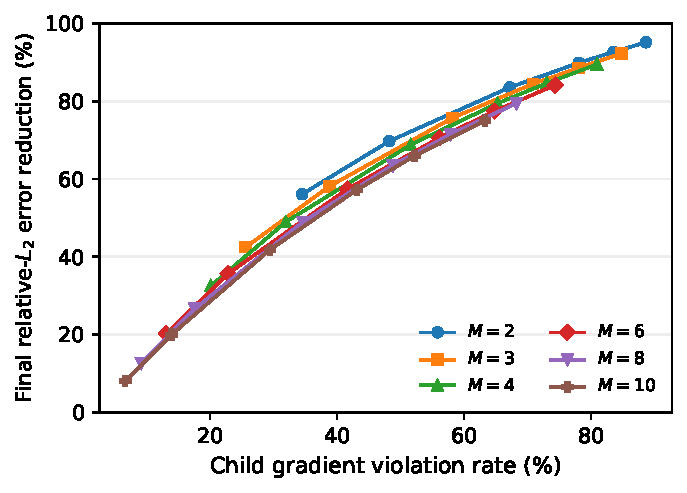
\includegraphics[width=.68\textwidth]{figures/restored/violation_gain_reproduction.pdf}
\caption{\textbf{Violation frequency complements overshoot energy.} The same newly executed 36 settings as Figure~\ref{fig:restored-mechanism}(a) are shown. Each line fixes $M$ and varies the certified radius from $1\times$ to $4\times$. Larger valid radii reduce the frequency of correction. Across the full shared-data sweep, the descriptive Spearman correlation is $0.995$.}
\label{fig:restored-violation}
\end{figure}
\FloatBarrier
\begin{table}[htbp]
\centering\small
\caption{All 36 settings of the independent, corrected-reference reproduction. $a$ multiplies the exact-matrix certificate $R_0$; $p$ is the pre-projection violation fraction. Raw and IR columns are mean relative $L_2$ errors over ten paired repetitions. These are newly sampled results, not reconstructed old figure coordinates.}\label{tab:restored-overshoot}
\begin{tabular}{rrrrrrr}
\toprule
$M$ & $a$ & $\widehat\Omega$ & $p$ (\%) & Raw & IR & Gain (\%) \\
\midrule
2 & 1 & 205.627 & 88.64 & 14.7731 & 0.7180 & 95.14 \\
2 & 1.25 & 188.722 & 83.54 & 14.7731 & 1.0826 & 92.67 \\
2 & 1.5 & 173.139 & 78.09 & 14.7731 & 1.4973 & 89.86 \\
2 & 2 & 145.591 & 67.18 & 14.7731 & 2.4311 & 83.54 \\
2 & 3 & 102.620 & 48.22 & 14.7731 & 4.4727 & 69.72 \\
2 & 4 & 71.954 & 34.48 & 14.7731 & 6.4891 & 56.07 \\
\midrule
3 & 1 & 127.685 & 84.83 & 8.9572 & 0.6925 & 92.27 \\
3 & 1.25 & 114.912 & 78.01 & 8.9572 & 1.0260 & 88.55 \\
3 & 1.5 & 103.372 & 70.86 & 8.9572 & 1.3918 & 84.46 \\
3 & 2 & 83.548 & 58.21 & 8.9572 & 2.1738 & 75.73 \\
3 & 3 & 54.292 & 38.77 & 8.9572 & 3.7509 & 58.12 \\
3 & 4 & 34.961 & 25.60 & 8.9572 & 5.1545 & 42.45 \\
\midrule
4 & 1 & 88.555 & 80.94 & 6.3795 & 0.6722 & 89.46 \\
4 & 1.25 & 78.243 & 73.02 & 6.3795 & 0.9806 & 84.63 \\
4 & 1.5 & 69.086 & 65.28 & 6.3795 & 1.3105 & 79.46 \\
4 & 2 & 53.756 & 51.60 & 6.3795 & 1.9895 & 68.81 \\
4 & 3 & 32.246 & 31.89 & 6.3795 & 3.2594 & 48.91 \\
4 & 4 & 18.991 & 20.12 & 6.3795 & 4.3045 & 32.53 \\
\midrule
6 & 1 & 52.753 & 74.33 & 3.9715 & 0.6299 & 84.14 \\
6 & 1.25 & 45.298 & 64.82 & 3.9715 & 0.8959 & 77.44 \\
6 & 1.5 & 38.870 & 56.12 & 3.9715 & 1.1678 & 70.59 \\
6 & 2 & 28.553 & 41.63 & 3.9715 & 1.6907 & 57.43 \\
6 & 3 & 15.189 & 22.82 & 3.9715 & 2.5561 & 35.64 \\
6 & 4 & 7.810 & 13.11 & 3.9715 & 3.1664 & 20.27 \\
\midrule
8 & 1 & 35.913 & 68.24 & 2.8884 & 0.5929 & 79.47 \\
8 & 1.25 & 30.094 & 57.88 & 2.8884 & 0.8243 & 71.46 \\
8 & 1.5 & 25.191 & 48.81 & 2.8884 & 1.0526 & 63.56 \\
8 & 2 & 17.583 & 34.60 & 2.8884 & 1.4739 & 48.97 \\
8 & 3 & 8.355 & 17.59 & 2.8884 & 2.1187 & 26.65 \\
8 & 4 & 3.757 & 9.14 & 2.8884 & 2.5227 & 12.66 \\
\midrule
10 & 1 & 26.444 & 63.31 & 2.2462 & 0.5609 & 75.03 \\
10 & 1.25 & 21.696 & 52.19 & 2.2462 & 0.7658 & 65.91 \\
10 & 1.5 & 17.776 & 43.10 & 2.2462 & 0.9614 & 57.20 \\
10 & 2 & 11.867 & 29.41 & 2.2462 & 1.3078 & 41.78 \\
10 & 3 & 5.106 & 13.92 & 2.2462 & 1.7975 & 19.98 \\
10 & 4 & 2.032 & 6.64 & 2.2462 & 2.0655 & 8.04 \\
\bottomrule
\end{tabular}
\end{table}

All value arrays, evaluation points, the matrix, references, per-repetition energies and rates, and summarized rows are included with the reproduction script. No coordinates were digitized from a figure.
\FloatBarrier

\section{Additional Positive Benchmarks and Geometry Ablations}
\label{app:recovered-benchmarks}
The older benchmark records answer questions not replaced by the three-method Batch-IR extension. The corrected HJB comparison in Figure~\ref{fig:benchmarks}(a) tests certified joint geometry against coordinate clipping and heuristic clipping. The two-budget Neufeld--Wu curves in Figure~\ref{fig:restored-mechanism}(b) and Table~\ref{tab:nw-extra} test an independent gradient-dependent implementation. Their archived 30-run records have been recovered; all six dimension--budget pairs, including the coordinate-box ties, are retained. The box and joint projection agree in value in this thresholded problem, so these results cannot establish that a ball is superior to a box for every generator.

\subsection{The Original Funding Work Curve and Higher-Level Geometry}
Figure~\ref{fig:finance-budget} retains the original budget-envelope image. Table~\ref{tab:restored-funding-budget} gives every recorded setting behind it, and Figure~\ref{fig:restored-funding-geometry}(a) plots all settings without replacing them by a running minimum. In particular, the projected method has MAE $0.4953$ at 220 generator calls; the raw method still has MAE $1.0996$ at 2,384 calls in this recorded sweep. These are benchmark-specific observations, not a cost-to-accuracy theorem or a wall-clock speedup.

The separate higher-level ablation in Figure~\ref{fig:restored-funding-geometry}(b) reaches depth five and keeps the coordinate-box control. At $(n,M)=(4,3)$, the raw, box, and joint-IR MAEs are $3.0252$, $2.7077$, and $0.8772$; at $(5,2)$ they are $5.1956$, $4.5922$, and $1.4590$. Hence the positive evidence is not restricted to the shallow root or to a comparison against an entirely unprotected method. The methods are paired within each row. The three settings have different budgets and replication counts; a depth-only trend is not inferred.

\begin{figure}[htbp]
\centering
\begin{subfigure}[t]{.485\textwidth}
\centering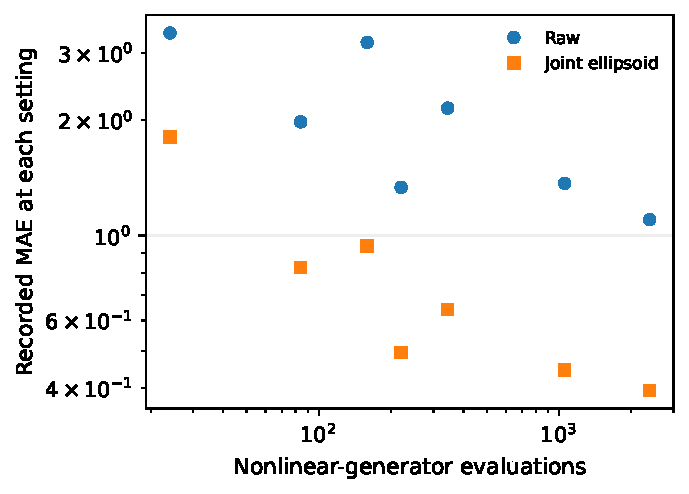
\includegraphics[width=\linewidth]{figures/restored/funding_all_budget_points.pdf}
\caption{Every recorded work/error setting.}
\end{subfigure}\hfill
\begin{subfigure}[t]{.485\textwidth}
\centering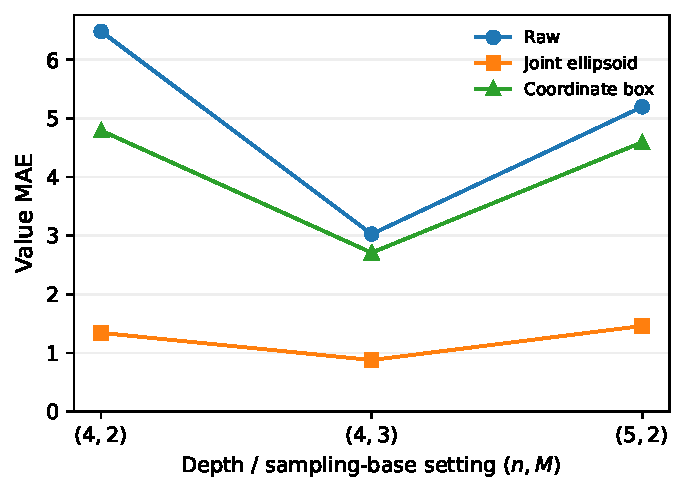
\includegraphics[width=\linewidth]{figures/restored/funding_deep_geometry.pdf}
\caption{Depths four and five: joint region versus box.}
\end{subfigure}
\caption{\textbf{Funding evidence not subsumed by the new Batch-IR comparison.} (a) Dots show all seven original settings; the original cumulative envelope is separately preserved in Figure~\ref{fig:finance-budget}. (b) A paired older geometry ablation includes the coordinate box and a fifth-level calculation. No Batch-IR series is spliced into these earlier experiments. The connecting lines in (b) only organize settings, not a continuous work or depth axis.}
\label{fig:restored-funding-geometry}
\end{figure}
\begin{table}[htbp]
\centering\small
\caption{All recorded settings behind the original funding work envelope. Counts are nonlinear-generator evaluations; replication counts differ across settings.}\label{tab:restored-funding-budget}
\begin{tabular}{rrrrrr}
\toprule
$n$ & $M$ & Runs & $f$ calls & Raw MAE & Joint IR MAE \\
\midrule
2 & 3 & 100 & 24 & 3.3759 & 1.8063 \\
2 & 6 & 100 & 84 & 1.9789 & 0.8253 \\
2 & 10 & 100 & 220 & 1.3357 & 0.4953 \\
3 & 3 & 100 & 159 & 3.1904 & 0.9393 \\
3 & 4 & 100 & 344 & 2.1495 & 0.6413 \\
3 & 6 & 60 & 1056 & 1.3686 & 0.4459 \\
3 & 8 & 40 & 2384 & 1.0996 & 0.3941 \\
\bottomrule
\end{tabular}
\end{table}

\begin{table}[htbp]
\centering\small
\caption{Earlier higher-level funding geometry ablation. The three methods are paired within each setting; no Batch-IR series is inferred from these data.}\label{tab:restored-funding-geometry}
\begin{tabular}{rrrrrrr}
\toprule
$n$ & $M$ & Runs & $f$ calls & Raw & Joint IR & Box \\
\midrule
4 & 2 & 60 & 252 & 6.4827 & 1.3411 & 4.7908 \\
4 & 3 & 30 & 1032 & 3.0252 & 0.8772 & 2.7077 \\
5 & 2 & 30 & 1124 & 5.1956 & 1.4590 & 4.5922 \\
\bottomrule
\end{tabular}
\end{table}

\FloatBarrier

\subsection{Mean Feasibility and the Earlier Thresholded-Driver Comparison}
The earlier batch study includes two further diagnostics. In the funding sweep, the mean-preserving rule is feasible in 0\%, 100\%, and 100\% of recorded runs at $M=10,20,40$. This concerns that diagnostic's feasible-mean condition, not the fraction of individual children inside the set. At $n=M=3$ in Neufeld--Wu, the mean-preserving rule coincides with raw MLP, whereas Samplewise IR and Batch-IR have identical lower MAEs. These are separate results from the $n=M=2$ extension in Appendix~\ref{app:extended-nw}.

\begin{figure}[htbp]
\centering
\begin{subfigure}[t]{.485\textwidth}
\centering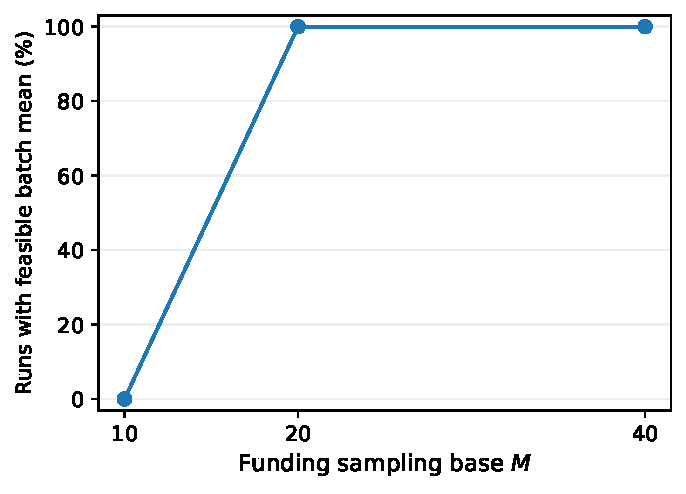
\includegraphics[width=\linewidth]{figures/restored/mean_preserving_feasibility.pdf}
\caption{Funding: feasible mean for the diagnostic.}
\end{subfigure}\hfill
\begin{subfigure}[t]{.485\textwidth}
\centering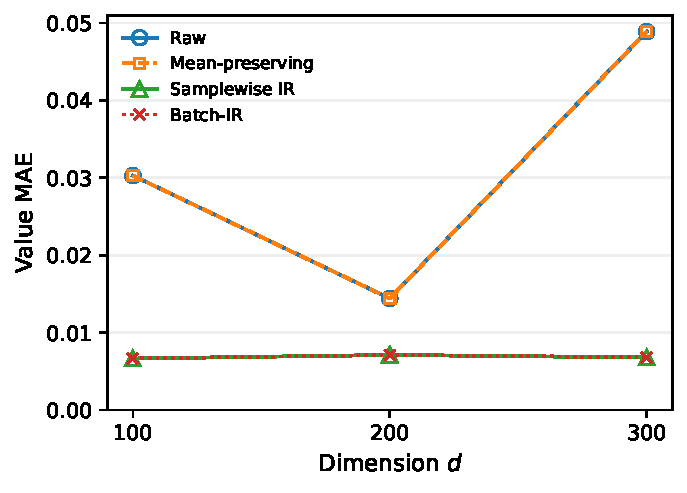
\includegraphics[width=\linewidth]{figures/restored/batch_neufeld_M3.pdf}
\caption{Neufeld--Wu: the earlier $n=M=3$ batch study.}
\end{subfigure}
\caption{\textbf{Feasibility and ties are part of the evidence.} Reported aggregate values are re-plotted without invented replication-level uncertainty. In (b), distinct markers expose two exact overlaps: Raw with the mean-preserving diagnostic, and Samplewise IR with Batch-IR. Preventing the same threshold activation gives a tie, not a Batch-IR win.}
\label{fig:restored-batch-controls}
\end{figure}
\FloatBarrier

\section{Controlled Surrogate-Quality Diagnostic}
\label{app:surrogate-diagnostic}
An archived 20D logistic test probes total-state constraints in a defect-correction setting. We retain it as a \emph{controlled diagnostic}, not as a comparison against trained SCaSML checkpoints. The surrogate is defined from the analytic solution as $\widehat u=q u^\star$, with $q\in\{1,0.95,0.75,0.5,0\}$. Its relative error is $1-q$. At depth $n=2$, three sampling bases $M\in\{1,2,4\}$ are tested with 40 repetitions for each setting. The methods are raw defect MLP, fixed defect clipping to $[-0.01,0.01]$, and correction using the total-state bounds $0\le u\le1$, $0\le z_i\le1/16$ recorded for this logistic test.

The noisiest budget illustrates why a fixed small defect range is not robust to surrogate quality. With no surrogate ($q=0$, $M=1$), raw and total-state-IR relative errors are $19.87\%$ and $18.37\%$, whereas fixed defect clipping gives $98.44\%$. The true correction is no longer small enough for the chosen defect clip. This does not establish that total-state IR always helps: at $M=4$ it is worse than raw defect MLP at every nonperfect surrogate setting in the archive. For example, at 25\% surrogate error the errors are $1.357\%$ (raw) and $1.714\%$ (IR). All such rows are included in Table~\ref{tab:restored-surrogate}.

\begin{figure}[htbp]
\centering
\begin{subfigure}[t]{.485\textwidth}
\centering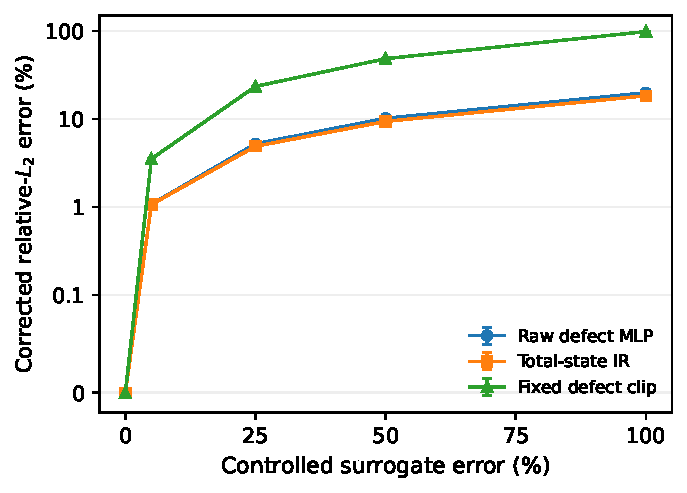
\includegraphics[width=\linewidth]{figures/restored/surrogate_quality_M1.pdf}
\caption{Sampling base $M=1$.}
\end{subfigure}\hfill
\begin{subfigure}[t]{.485\textwidth}
\centering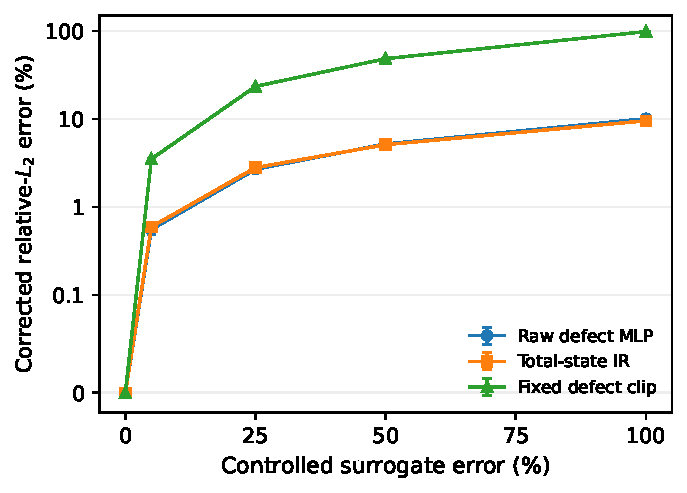
\includegraphics[width=\linewidth]{figures/restored/surrogate_quality_M2.pdf}
\caption{Sampling base $M=2$.}
\end{subfigure}
\caption{\textbf{A fixed defect clip is sensitive to surrogate quality.} The surrogate is analytically scaled, not trained. Error bars are the recorded standard deviations over 40 runs, not confidence intervals. The vertical axis is symmetric-log with a linear segment below 0.1 percentage point, retaining the exact zero-error perfect-surrogate case.}
\label{fig:restored-surrogate12}
\end{figure}
\begin{figure}[htbp]
\centering
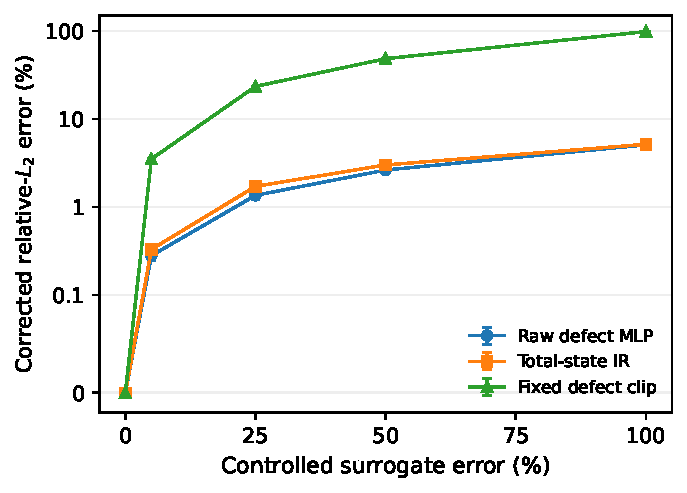
\includegraphics[width=.58\textwidth]{figures/restored/surrogate_quality_M4.pdf}
\caption{\textbf{The larger-budget boundary case is retained.} At $M=4$, raw defect MLP is already sufficiently accurate that total-state correction has no general advantage and slightly worsens the nonperfect cases. This panel uses the same axis convention and uncertainty definition as Figure~\ref{fig:restored-surrogate12}. It is not evidence against the exact counterexample theorem, which concerns a different generator and constraint.}
\label{fig:restored-surrogate4}
\end{figure}
\FloatBarrier
\begin{table}[htbp]
\centering\small
\caption{Controlled logistic-surrogate diagnostic: relative $L_2$ error in percent (mean $\pm$ recorded standard deviation over 40 runs). The perfect-surrogate rows remain, and the table also retains cases where IR is worse than raw defect MLP.}\label{tab:restored-surrogate}
\begin{tabular}{rrccc}
\toprule
$M$ & Surrogate error (\%) & Raw defect MLP & Total-state IR & Fixed defect clip \\
\midrule
1 & 0 & $0.000\pm0.000$ & $0.000\pm0.000$ & $0.000\pm0.000$ \\
1 & 5 & $1.073\pm0.075$ & $1.067\pm0.062$ & $3.524\pm0.004$ \\
1 & 25 & $5.221\pm0.301$ & $4.898\pm0.252$ & $23.453\pm0.001$ \\
1 & 50 & $10.178\pm0.518$ & $9.382\pm0.461$ & $48.446\pm0.000$ \\
1 & 100 & $19.865\pm1.037$ & $18.368\pm0.888$ & $98.444\pm0.000$ \\
\midrule
2 & 0 & $0.000\pm0.000$ & $0.000\pm0.000$ & $0.000\pm0.000$ \\
2 & 5 & $0.555\pm0.063$ & $0.594\pm0.044$ & $3.512\pm0.001$ \\
2 & 25 & $2.684\pm0.234$ & $2.804\pm0.131$ & $23.452\pm0.000$ \\
2 & 50 & $5.202\pm0.341$ & $5.105\pm0.238$ & $48.446\pm0.000$ \\
2 & 100 & $10.077\pm0.512$ & $9.541\pm0.450$ & $98.444\pm0.000$ \\
\midrule
4 & 0 & $0.000\pm0.000$ & $0.000\pm0.000$ & $0.000\pm0.000$ \\
4 & 5 & $0.280\pm0.035$ & $0.330\pm0.022$ & $3.510\pm0.000$ \\
4 & 25 & $1.357\pm0.136$ & $1.714\pm0.112$ & $23.452\pm0.000$ \\
4 & 50 & $2.630\pm0.206$ & $3.005\pm0.207$ & $48.446\pm0.000$ \\
4 & 100 & $5.089\pm0.346$ & $5.159\pm0.362$ & $98.444\pm0.000$ \\
\bottomrule
\end{tabular}
\end{table}

The archived JSON supplies 45 method-level rows, including the perfect surrogate and all three budgets. No learned-checkpoint training cost, real-surrogate generalization result, or end-to-end SCaSML superiority is inferred from these data.
\FloatBarrier

\section{Batchwise Negative Controls}
\label{app:restored-negative}
The repository's paired negative-control suite complements the earlier samplewise controls. It separates two reasons for an absent value benefit: the constraint can be inactive, or it can be active on a state that is irrelevant to the generator. Figure~\ref{fig:restored-inactive-controls} and Table~\ref{tab:restored-negative} preserve both methods' overlaps rather than omit zero-gain cases.

\begin{table}[htbp]
\centering\small
\caption{Recorded paired negative controls. All three methods have the same error and zero maximum value discrepancy. Allen--Cahn reports relative MAE in percent; the other rows report absolute MAE. Activity columns refer to the constrained state and the Batch-IR implementation.}\label{tab:restored-negative}
\begin{tabular}{lrrrrrr}
\toprule
Problem & $n$ & $M$ & Common error & Violation (\%) & Batch active (\%) & Max $\Delta u$ \\
\midrule
Allen--Cahn & 3 & 2 & 3.303465 & 0.00 & 0.00 & 0 \\
Allen--Cahn & 3 & 3 & 1.959025 & 0.00 & 0.00 & 0 \\
Allen--Cahn & 3 & 4 & 1.421529 & 0.00 & 0.00 & 0 \\
\midrule
Credit risk & 2 & 10 & 0.450018 & 0.00 & 0.00 & 0 \\
Credit risk & 3 & 6 & 0.297810 & 0.00 & 0.00 & 0 \\
Credit risk & 4 & 3 & 0.516940 & 0.00 & 0.00 & 0 \\
\midrule
Linear & 2 & 4 & 0.114882 & 100.00 & 100.00 & 0 \\
Linear & 2 & 8 & 0.050744 & 97.00 & 97.00 & 0 \\
Linear & 2 & 16 & 0.026660 & 8.50 & 8.50 & 0 \\
\bottomrule
\end{tabular}
\end{table}


\subsection{Inactive Constraints: Allen--Cahn and Credit Risk}
For 100D Allen--Cahn, $n=3$ and $M=2,3,4$ use the maximum-principle interval $[0,1]$ with 100 paired repetitions. No child violates the interval, and Batch-IR uses $\alpha_B=1$ throughout. Raw, Samplewise IR, and Batch-IR match realization by realization. The earlier Allen--Cahn panel in Figure~\ref{fig:allen-control} remains; the new panel explicitly includes Batch-IR.

For the 100D credit-risk experiment, the recorded parameters are $T=2$, $\sigma=0.2$, $\beta=0.03$, $K_1=30$, $K_2=60$, $L=15$, and reference value 2.626. The tested interval is $[-15,15]$. Each setting has 100 paired repetitions, and all methods again match exactly with zero constraint activity. These values belong to the newer paired negative-control run and are not substituted for the earlier credit-risk seed set.

\begin{figure}[htbp]
\centering
\begin{subfigure}[t]{.485\textwidth}
\centering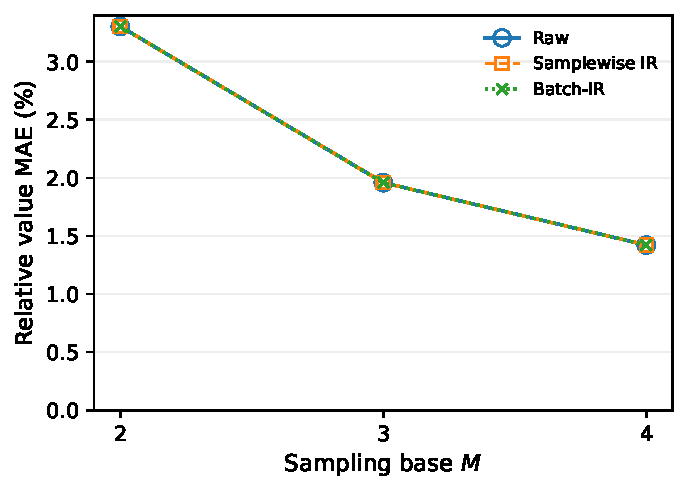
\includegraphics[width=\linewidth]{figures/restored/negative_allen_batch.pdf}
\caption{Allen--Cahn: relative MAE in percent.}
\end{subfigure}\hfill
\begin{subfigure}[t]{.485\textwidth}
\centering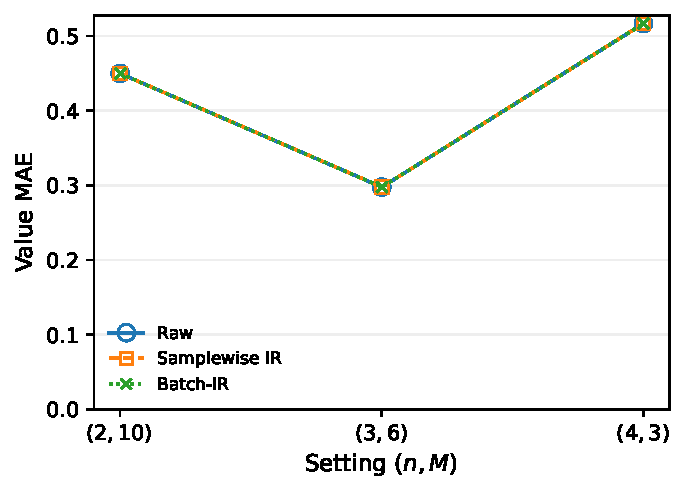
\includegraphics[width=\linewidth]{figures/restored/negative_credit_batch.pdf}
\caption{Credit risk: absolute MAE.}
\end{subfigure}
\caption{\textbf{Inactive constraints leave all three algorithms unchanged.} Open and crossed markers expose identical curves without horizontal jitter or artificial separation. Every recorded maximum value difference from raw MLP is zero. The credit-risk settings vary both depth and sampling base.}
\label{fig:restored-inactive-controls}
\end{figure}
\FloatBarrier

\subsection{Active but Generator-Irrelevant Gradient Correction}
For the linear 100D convection--diffusion test, $f=0$. The noisy gradient estimate is corrected, but the value estimator does not depend on that gradient. At $M=4,8,16$, the recorded gradient-violation and batch-activation rates are 100\%, 97\%, and 8.5\%, respectively. Nevertheless the paired value outputs remain exactly identical. This is stronger than an inactive-constraint control: feasibility correction can occur frequently without improving a value that never reuses the constrained channel.

\begin{figure}[htbp]
\centering
\begin{subfigure}[t]{.485\textwidth}
\centering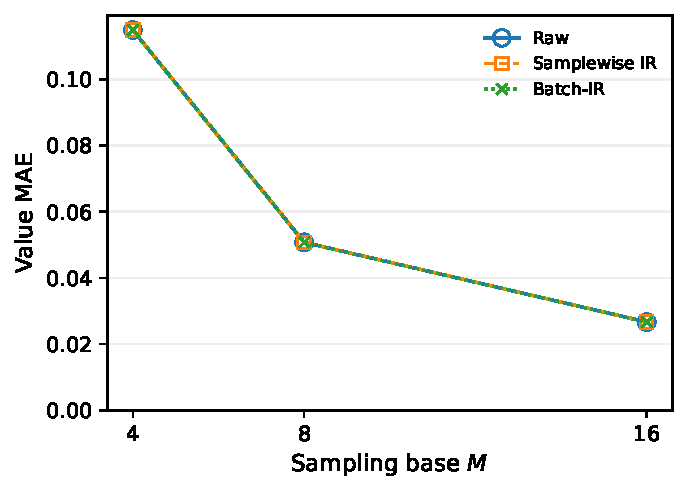
\includegraphics[width=\linewidth]{figures/restored/negative_linear_batch.pdf}
\caption{Value error is unchanged.}
\end{subfigure}\hfill
\begin{subfigure}[t]{.485\textwidth}
\centering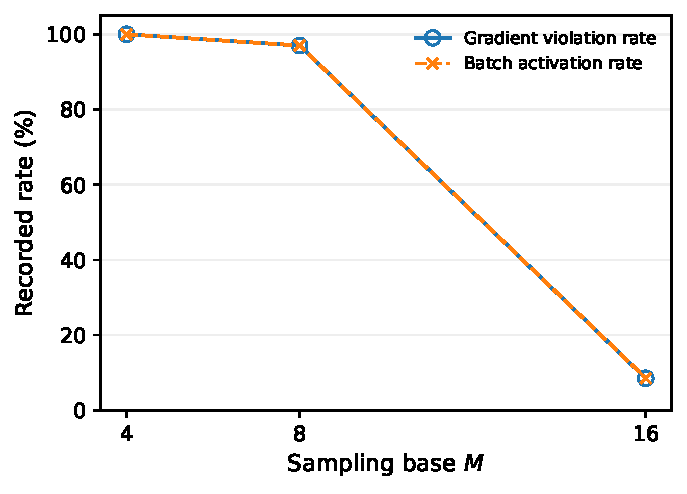
\includegraphics[width=\linewidth]{figures/restored/negative_linear_activity.pdf}
\caption{The gradient correction is nevertheless active.}
\end{subfigure}
\caption{\textbf{Constraint activity alone is not the mechanism.} (a) All methods have equal value MAE and zero maximum paired discrepancy. (b) Gradient-violation and Batch-IR activation rates overlap but are often large. Because $f=0$, the corrected gradient cannot affect the value path.}
\label{fig:restored-active-control}
\end{figure}
\FloatBarrier

\section{An Elliptic Neural-BSDE Diagnostic Outside the MLP Claim}
\label{app:elliptic-diagnostic}
For completeness, the older repository also records a diagnostic on the semilinear elliptic benchmark of \citet{Kremsner2020}. This uses a neural random-terminal-time BSDE solver, \emph{not} an MLP recursion, and is not counted as an additional positive MLP benchmark. On the unit ball the equation and analytic solution are
\[
 \Delta u+\norm{\nabla u}^2=2e^{-u},\quad
 u|_{\partial B}=\log(2/d),\qquad
 u(x)=\log\!\left(\frac{1+\norm x^2}{d}\right),\quad
 \nabla u(x)=\frac{2x}{1+\norm x^2}.
\]
Thus $\norm{\nabla u}\le1$ is a valid ball certificate. The run uses $d=100$, simulated horizon 0.1, 50 time intervals, 500 Adam iterations, training batches of 64, validation size 256, and a starting point of radius 0.5.

The baseline implementation divides the gradient-network output by $d$. Under this scaling, the radius-one projection is inactive and the tested corrections coincide. Removing only this scaling produces a useful but mixed ablation. Across three paired seeds, the joint ball lowers the terminal squared BSDE residual from 0.0275 to 0.0103, but slightly raises the relative error of the one reported value from 1.76\% to 1.80\%. The coordinate box gives a smaller value error while substantially worsening the terminal loss (Table~\ref{tab:restored-elliptic}). Neither metric should be hidden in favor of the other.

\begin{figure}[htbp]
\centering
\begin{subfigure}[t]{.485\textwidth}
\centering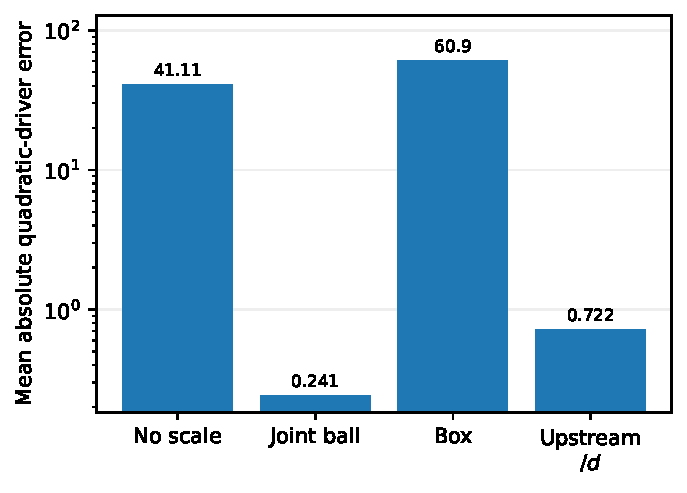
\includegraphics[width=\linewidth]{figures/restored/elliptic_driver_diagnostic.pdf}
\caption{Mean absolute quadratic-driver error, seed 0.}
\end{subfigure}\hfill
\begin{subfigure}[t]{.485\textwidth}
\centering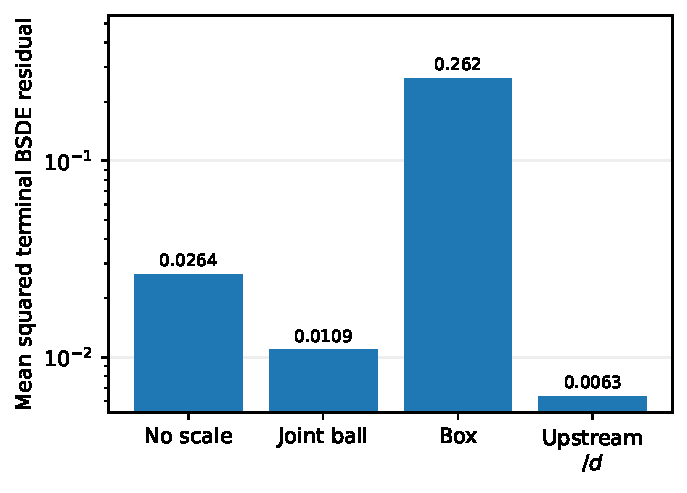
\includegraphics[width=\linewidth]{figures/restored/elliptic_terminal_diagnostic.pdf}
\caption{Terminal squared BSDE residual, seed 0.}
\end{subfigure}
\caption{\textbf{Different metrics can favor different corrections.} These are archived seed-0 diagnostics, not averages over three seeds. The driver statistic is the mean of $|\norm{\widehat z}^2-\norm{\nabla u}^2|$ on active sampled states; it is not generator MSE. The upstream $/d$ rule remains best on terminal loss. This out-of-scope extension is retained as a limitation/diagnostic, not presented as an improvement over the published elliptic solver.}
\label{fig:restored-elliptic}
\end{figure}
\begin{table}[htbp]
\centering\small
\caption{Archived elliptic no-scale ablation, means over three paired seeds. Lower terminal loss does not imply lower error in the single reported value. Rounded report values are preserved. This is a neural BSDE diagnostic, not an MLP benchmark.}\label{tab:restored-elliptic}
\begin{tabular}{lrr}
\toprule
Method & Relative value error (\%) & Terminal BSDE loss \\
\midrule
No scale & 1.76 & 0.0275 \\
Joint ball & 1.80 & 0.0103 \\
Coordinate box & 0.53 & 0.2682 \\
\bottomrule
\end{tabular}
\end{table}

In the archived seed-0 radius check, terminal losses are 0.0109, 0.0275, and 0.1020 at ball radii 1, 2, and 4. Relaxing the certified bound weakens this pathwise stabilization, but does not turn it into a theorem about the trained solver or the reported value error. These figures use the rounded source-report values; no new neural training was performed for this manuscript update.
\FloatBarrier
